\chapter{Séance 2: mardi 18 décembre 2018}
Dans cette séance, on revient d'abord sur la notion de Markov-compatibilité: on donne entre autres deux caractérisations, qui sont sans doute plus parlantes que la définition. Dans une seconde partie, on introduit les modèles causaux \emph{fonctionnels}, qui sont une façon alternative aux CBN de se donner une distribution et des liens de causalité. Ces modèles fonctionnels vont nous permettre de répondre aux \emph{questions contrefactuelles}.

On rappelle la notion d'indépendance conditionnelle qui va intervenir
dans une des caractérisations de la Markov-compatibilité.

\begin{definition}[Indépendance conditionnelle]
Soit $P$ une distribution pour $V$.
Soit $X,Y,Z\subset V$ des sous-ensembles de variables.
On dit que $X$ et $Y$ sont indépendants conditionnellement à $Z$ pour la distribution $P$ si:
  \[ P(x|y,z)=P(x|z)  \]
dès que les quantités ci-dessus existent, c'est-à-dire dès que $P(y,z)>0$. On note alors $(X\indep Y|Z)_P$.
\end{definition}
Autrement dit, ayant observé $Z$, l'observation supplémentaire de $Y$ ne modifie pas la loi de $X$.

\section{$d$-séparation}
\label{sec:d-separation}
La $d$-séparation est une notion portant sur la \emph{structure d'un
  graphe}. Elle permet de déduire des propriétés sur les distributions
de probabilité Markov-compatibles avec le graphe.
La notion sera utilisée dans la Section~\ref{sec:caract-de-la} pour
établir des caractérisations de la Markov-compatibilité.
\begin{definition}
On appelle chemin (sous-entendu non-orienté) de $X$ à $Y$ une suite de
n\oe uds $(X=V_1,\dots,V_k=Y)$ tous différents tels que pour tout $i\in \left\{ 1,\dots,k-1 \right\}$:
\[ V_i\to V_{i+1}\qquad \text{ou}\qquad V_i\leftarrow V_{i+1}. \]
\end{definition}
\begin{example}
$X\to Z\leftarrow Y$ est un chemin de $X$ à $Y$.
\end{example}

\begin{definition}[$d$-séparation]
  \label{def:d-separation}
Soit $G$ un graphe orienté sur $V$, et $X,Y,Z\subset V$ des sous-ensembles
disjoints de n\oe uds.
On dit qu'un chemin $p$ est $d$-séparé (ou bloqué) par l'ensemble de
n\oe ud $Z$ si le chemin $p$ contient:
\begin{enumerate}[(I)]
\item\label{item:d-sep-I} un n\oe ud dans $Z$,
\item\label{item:d-sep-II} ou une configuration de la forme:
   \[ i\to \underbrace{X_0}_{\not \in Z}\leftarrow j \]
   tel qu'aucun descendant de $X_0$ n'est dans $Z$.
\end{enumerate}
On dit que $Z$ $d$-sépare $X$ et $Y$ si $Z$ $d$-sépare tous les
chemins de $X$ à $Y$. On note alors $(X\indep Y|Z)_G$.
\end{definition}
\begin{example}
On considère le graphe de l'exemple du Sol mouillé (Section~\ref{sec:exemple-intr-ii}).
\begin{center}
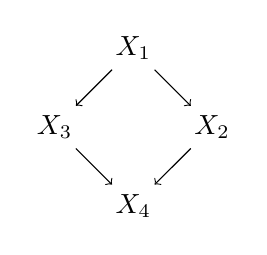
\begin{tikzpicture}[scale=1]
\node (X1) at (0,2) {$X_1$};
\node (X2) at (1,1) {$X_2$};
\node (X3) at (-1,1) {$X_3$};
\node (X4) at (0,0) {$X_4$};
\draw[->] (X1) -- (X2);
\draw[->] (X2) -- (X4);
\draw[->] (X1) -- (X3);
\draw[->] (X3) -- (X4);
\end{tikzpicture}
\end{center}
On peut voir que $X_1$ $d$-sépare $X_3$ et $X_2$. En effet, il existe
2 chemins de $X_3$ à $X_2$, qui sont $X_3\leftarrow X_1\to X_2$ et $X_3\to X_4\leftarrow X_2$.
Le premier chemin est $d$-séparé par $X_1$ car il contient $X_1$ (cas
(\ref{item:d-sep-I})). Le second chemin est aussi $d$-séparé par $X_1$
car il contient $\to X_4\leftarrow$ et qu'aucun descendant de $X_4$ n'est dans $\left\{ X_1 \right\}$ (cas (\ref{item:d-sep-II})).
En revanche, $X_4$ ne $d$-sépare pas $X_2$ et $X_3$ car le chemin
$X_2\leftarrow X_1\to X_3$ ne satisfait ni (\ref{item:d-sep-I}) ni (\ref{item:d-sep-II}).
\end{example}
Le résultat suivant établit le lien entre $d$-séparation,
Markov-compatbilité et indépendance conditionnelle.
\begin{theorem}[\cite{verma1988causal}]
\label{thm:d-separation-markov-compatibilite}
Soit $G$ un DAG sur $V$, et $X,Y,Z\subset V$ des sous-ensembles disjoints de variables.
On a:
   \[ (X\indep Y|Z)_G\quad \Longleftrightarrow \quad \forall P \text{ compatible avec }G,\quad  (X\indep Y|Z)_P. \]
\end{theorem}

\section{Caractérisations de la Markov-compatibilité}
\label{sec:caract-de-la}

\begin{definition}
Soit $G$ un graphe orienté sur $V$. On dit que qu'une numérotation des
variables $V=(X_1,\dots,X_n)$ est \emph{compatible} avec (les
arêtes de) $G$ si \[ X_i\to X_j\quad \Longrightarrow \quad i<j. \]
\end{definition}
\begin{example}
  On considère le graphe:  $X_3\leftarrow X_1\to X_2\to X_4$; la numérotation et le graphe sont compatibles.
\end{example}
\begin{proposition}
Soit $G$ un graphe orienté sur $V$. $G$ est acyclique si et seulement
si il existe une numérotation des n\oe uds $V=(X_1,\dots,X_n)$
compatible avec $G$.
\end{proposition}
\begin{definition}
Soit $X,Y\in V$ et $G$ un graphe orienté sur $V$. On dit que $Y$ est un \emph{non-descendant} de
$X$ dans $G$ si $Y\neq X$ et s'il n'existe pas de chemin orienté de la forme $X\to \dots \to Y$.
\end{definition}
\begin{theorem}[Caractérisations de la Markov-compatibilité]
\label{thm:caracterisations-markov-compatibilite}
Soit $P$ une distribution pour $V$ et $G$ un DAG sur $V$. Les trois propositions suivantes sont équivalentes.
\begin{enumerate}[(i)]
\item\label{item:P-G-compatibles} $P$ et $G$ sont Markov-compatibles.
\item\label{item:omc} (Ordered Markov Condition) Il existe une numérotation des variables $V=(X_i)_{1\leqslant i\leqslant n}$ compatible avec $G$ et telle que:
\begin{equation}
\label{eq:omc}
i<j\quad \Longrightarrow \quad (X_i\indep X_j|PA_j)_P.
\end{equation}
\item\label{item:pmc} (Parental Markov Condition) Pour tous $X,Y\in V$:
\[ Y\text{ non-descendant de }X\quad \Longrightarrow \quad (X\indep Y|PA_X)_P. \]
\end{enumerate}
\end{theorem}
\begin{proof}
(\ref{item:pmc}) $\Longrightarrow$ (\ref{item:omc}). On suppose la Parental Markov Condition. 
$G$ étant un DAG, il existe une numérotation des variables qui soit compatible avec $G$. 
Pour une telle numérotation, $i<j$ implique que $X_i$ est un non-descendant de $X_j$, et on a donc $(X_i\indep X_j|PA_j)$ grâce à la Parental Markov Condition.

(\ref{item:omc}) $\Longrightarrow$ (\ref{item:P-G-compatibles}).
Supposons que la Ordered Markov Condition est satisfaite. On considère une numérotation correspondante des variables.
Soit $v=(x_i)_{1\leqslant i\leqslant n}\in D_V$.
L'implication (\ref{eq:omc}) entraîne que pour tout $i\in \left\{ 1,\dots,n \right\}$:
\[ P(x_i|pa_i)=P(x_i|x_1,\dots,x_{i-1},pa_i). \] 
La compatibilité de la numérotation des variables avec $G$ implique que les parents de $X_i$ ne peuvent être que parmi les variables précédentes, autrement dit:  $PA_i\subset (X_1,\dots,X_{i-1})$. L'égalité ci-dessus se simplifie donc en:
\[ P(x_i|pa_i)=P(x_i|x_1,\dots,x_{i-1}). \]
En injectant cette relation dans la suivante qui est toujours vraie:
\[ P(x_1,\dots,x_n)=\prod_{i=1}^nP(x_i|x_1,\dots,x_{i-1}), \]
on obtient bien la factorisation qui définit la Markov-compatibilité (Définition~\ref{def:markov-compatibilite}):
\[ P(x_1,\dots,x_n)=\prod_{i=1}^nP(x_i|pa_i). \]

(\ref{item:P-G-compatibles}) $\Longrightarrow$ (\ref{item:pmc}). Supposons que $P$ et $G$ sont Markov-compatibles.
Soit $X,Y\in V$ tels que $Y$ est un non-descendant de $X$ et $p$ un chemin entre $X$ et $Y$.
\begin{itemize}
\item Si $p$ contient une arête qui arrive sur $X$: ($\to X$), alors
  $p$ contient un n\oe ud dans $PA_X$, et $PA_X$  $d$-sépare
  le chemin $p$ (cas (\ref{item:d-sep-I}) de la Définition~\ref{def:d-separation}).
\item Sinon $p$ contient une arête qui part de $X$. Donc partant de
  $X$, on peut considérer $Z$ le premier n\oe ud qui est la
  destination de deux arêtes appartenant à $p$:
\[ X\to \dots \to Z\leftarrow \dots Y. \]
Un tel n\oe ud $Z$ existe bien car sinon on aurait $X\to \dots \to Y$
et $Y$ serait alors un descendant de $X$. De plus, $Z$ ne contient pas
de descendant dans $PA_X$ car on trouverait alors un cycle dans $G$ de
la forme:
\[ X\to \dots \to Z\to \dots \to \underbrace{W}_{\in PA_X}\to X. \]
Le chemin $p$ satisfait donc le cas (\ref{item:d-sep-II}) de la Définition~\ref{def:d-separation}, et $PA_X$  $d$-sépare bien $p$.
\end{itemize}
Ainsi, on a $(X\indep Y|PA_X)_G$ et donc $(X\indep Y|PA_X)_P$ grâce au Théorème~\ref{thm:d-separation-markov-compatibilite}.
\end{proof}

\begin{remark}[Ordered vs Parental Markov Condition]
Si l'on souhaite \emph{établir} la Markov-compatibilité, la
  Ordered Markov Condition est plus facile à vérifier,
  puisqu'il y a moins d'indépendance conditionnelles à
  vérifier: on peut voir en effet que toutes les indépendances conditionnelles de la Ordered Markov Condition sont contenues dans celles de la Parentel Markov Condition.

À l'inverse, si on \emph{sait} que $P$ et $G$ sont
  Markov-compatibles, alors la Parental Markov Condition du Theorème
  nous donne plus d'indépendances conditionnelles.
\end{remark}

\begin{definition}[$v$-structure]
Soit $G$ un graphe orienté sur $V$. Un triplet $(X,Y,Z)\in V^3$ est une $v$-structure de $G$ si:
\begin{itemize}
\item $X\to Z\leftarrow Y$
\item $X\not \to Y$
\item $Y\not \to X$.
\end{itemize}
\end{definition}
\begin{theorem}[Observational equivalence]
\label{thm:1}
Soit $G,G'$ deux DAG sur $V$.
$G$ et $G'$ ont la même classe de distributions Markov-compatibles
(on dit aussi sont "observationally equivalent") si, et seulement si
ils ont le même squelette et les mêmes v-structures, autrement dit:
si pour tous $X,Y,Z\in V$,
\begin{itemize}
\item $X\to_G Y\quad \Longleftrightarrow \quad X\to_{G'} Y$ ou $X\leftarrow_{G'} Y$
\item $(X,Y,Z)$ v-structure dans $G$ $\Longleftrightarrow$ $(X,Y,Z)$
  v-structure dans $G'$.
\end{itemize}
\end{theorem}

\begin{example}
  Si $V=\left\{ X,Y \right\}$, $G:X\to Y$, $G':X\leftarrow Y$ sont
  observationally equivalent. En effet, ils ont le mêm squelette et
  n'ont pas de $v$-structure. La donnée d'une distribution Markov-compatible ne permet pas de distinguer les deux graphes.
\end{example}

On peut malgré tout déduire certaines directions de flèches de la
distribution.
\begin{example}[Sol mouillé]
  On considère le DAG de l'exemple du sol mouillé:
\begin{center}
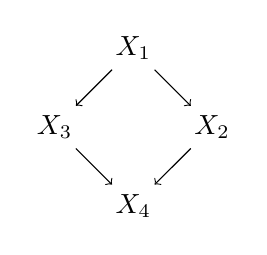
\begin{tikzpicture}[scale=1]
\node (X1) at (0,2) {$X_1$};
\node (X2) at (1,1) {$X_2$};
\node (X3) at (-1,1) {$X_3$};
\node (X4) at (0,0) {$X_4$};
\draw[->] (X1) -- (X2);
\draw[->] (X2) -- (X4);
\draw[->] (X1) -- (X3);
\draw[->] (X3) -- (X4);
\end{tikzpicture}
\end{center}
Changer le sens de l'arête $X_2\to X_4$ ou de l'arête
$X_3\to X_4$ supprime la $v$-structure $X_2\to X_4\leftarrow X_3$, et
donc modifie la classe de distributions compatibles. Donc si on est en
présence d'une distribution qui n'est Markov-compatible qu'avec l'un
des deux graphes, on peut déduire le sens de la flèche concernée.
\end{example}

\section{Modèles causaux sous forme fonctionnelle}
\label{sec:modeles-causaux-sous}

La donnée d'un CBN, c'est-à-dire la donnée de $P$ et de $G$
Markov-compatibles, nous a permis en Section~\ref{sec:la-distribution-p}  de définir la distribution \emph{modifiée par une intervention}. 

On va à présent introduire les \emph{modèles causaux fonctionnels}
(Functional Causal Models, FCM) qui sont une façon alternative de se
donner une distribution de probabilité et des liens de causalité.  Il
s'agit d'une représentation qui contient plus d'information que les
CBN, et qui vont permettre de répondre à des \emph{questions
  contrefactuelles} (qui sont introduites en
Section~\ref{sec:intr-aux-quest} ci-dessous), ce que ne permettait pas les CBN.

Un autre avantage des modèles \emph{fonctionnels} est qu'il vont
permettre (plus tard) de considérer des modèles \emph{cycliques}.

\begin{example}[Sol mouillé]
  \label{ex:sol-mouille-fcm}
La distribution $P$ de l'exemple du Sol mouillé pourrait être définie
de la façon suivante.
\begin{align*}
X_1&=U_1\qquad \text{avec }U_1\sim \mathcal{B}(1/2)\\
X_2&=\left\lceil \frac{X_1-1}{2}+U_2 \right\rceil \qquad \text{avec }U_2\sim \mathcal{U}(\left\{ 0,1/4,1/2,3/4 \right\})\\
X_3&=1-X_1\\
X_4&=\max_{}(X_2,X_3),
\end{align*}
et en supposant que les variables aléatoires $(U_1,U_2)$ sont
indépendantes. Cela définit une distribution jointe sur
$(X_1,\dots,X_4)$ qui est bien la même que celle de la Section~\ref{sec:exemple-intr-ii}.

D'une telle écriture \emph{fonctionnelle}, on peut également déduire
un graphe associé: pour chaque variable $X_i$, on définit ses parents
comme étant les variables $X_j$ apparaissant dans le membre de droite
correspondant. Le graphe associé à aux équations fonctionnelles
ci-dessus est le même que celui donné en Section~\ref{sec:exemple-intr-ii}.
\end{example}

\begin{definition}[Modèle causal fonctionnel (Functional Causal Model,
  FCM]
  Un \emph{modèle causal fonctionnel} (FCM) pour
  $V=(X_1,\dots,X_n)$ est la donnée pour tout $i\in \left\{ 1,\dots,n \right\}$:
\begin{itemize}
\item d'un sous-ensemble de variables $PA_i\subset V$,
\item d'une variable aléatoire $U_i$,
\item d'une fonction $f_i:D_{PA_i}\times D_{U_i}\to D_{X_i}$.
\end{itemize}
On note alors:
\begin{equation}
\label{eq:fcm}
X_i=f_i(PA_i,U_i),\quad i=1,\dots,n.
\end{equation}
Les variables $U_i$ sont appelées \emph{variables d'erreur}.
\end{definition}

\begin{definition}
  Soit $M$ un FCM pour $V=(X_1,\dots,X_n)$.
  Le graphe orienté $G$ (sur $V$) induit par $M$ est défini par:
\[ X_i\to_G X_j\quad \Longleftrightarrow X_i\in PA_j.  \]
\begin{itemize}
\item Si $G$ est acyclique, $M$ est dit \emph{semi-Markovien}.
\item Si e plus les variables $(U_1,\dots,U_n)$ sont indépendantes, $M$ est dit \emph{Markovien}.
\end{itemize}
\end{definition}
\begin{remark}
Si $M$ est semi-Markovien, la distribution des $(X_1,\dots,X_n)$ est
déterminée par la distribution de $(U_1,\dots,U_n)$, via les
équations \eqref{eq:fcm}.
\end{remark}
Si $M$ est Markovien, on peut dessiner $U_i$ sur le graphe avec
des poitillés. Par exemple, la forme fonctionnelle du Sol mouillé
(Exemple~\ref{ex:sol-mouille-fcm}) se représente comme suit.
\begin{center}
\begin{tikzpicture}[scale=1]
\node (U1) at (1,3) {$U_1$};
\node (X1) at (0,2) {$X_1$};
\node (U2) at (2,2) {$U_2$};
\node (X2) at (1,1) {$X_2$};
\node (X3) at (-1,1) {$X_3$};
\node (X4) at (0,0) {$X_4$};
\draw[->] (X1) -- (X2);
\draw[->] (X2) -- (X4);
\draw[->] (X1) -- (X3);
\draw[->] (X3) -- (X4);
\draw[->,dotted] (U1) -- (X1);
\draw[->,dotted] (U2) -- (X2);
\end{tikzpicture}
\end{center}
Si $M$ n'est pas Markovien, c'est-à-dire si les variables d'erreur
$(U_1,\dots,U_n)$ ne sont pas indépendantes, on les représente avec des
double-flèches entre les $U_i$.
\begin{center}
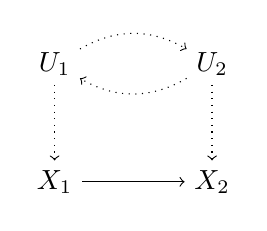
\begin{tikzpicture}[scale=1]
\node (X1) at (0,0) {$X_1$};
\node (U1) at (0,1.5) {$U_1$};
\node (X2) at (2,0) {$X_2$};
\node (U2) at (2,1.5) {$U_2$};
\draw[->] (X1) -- (X2);
\draw[->,dotted] (U1) -- (X1);

\draw[->,dotted] (U2) -- (X2);
\draw[->,dotted] (U1) to[bend left] (U2);
\draw[->,dotted] (U2) to[bend left]  (U1);
\end{tikzpicture}
\end{center}

\begin{proposition}
  Soit $M$ un FCM Markovien et $P$ la distribution induite, $G$ le
  graphe orienté induit. Alors $P$ et $G$ sont Markov-compatibles.
\end{proposition}

\begin{theorem}[\cite{druzdzel1993causality}]
\label{thm:exists-generating-fcm}
Pour tout CBN $(G,P)$, il existe un FCM qui le génère.
\end{theorem}



\begin{proposition}[Représentation fonctionnelle des interventions]
  \label{prop:intervention-fcm}
  Soit \[ X_i=f_i(PA_i,U_i),\qquad i=1,\dots,n \] un FCM Markovien sur
  $V=(X_1,\dots,X_n)$. On note $(G,P)$ le CBN induit.  Soit
  $X\subset V$ et $x\in D_X$.  Alors la distribution $P_{X=x}$ est
  induite par le le FCM modifié:
  \[ X_i= \begin{cases} x_i&\text{si $X_i\in X$}\\
      f_i(PA_i,U_i)&\text{sinon}. \end{cases} \]
\end{proposition}
\begin{example}[Le Sol mouillé]
 En reprenant l'Exemple~\ref{ex:sol-mouille-fcm}, on peut représenter
 la distribution $P_{X_3=0}$ de la façon suivante:
\begin{align*}
X_1&=U_1\qquad \text{avec }U_1\sim \mathcal{B}(1/2)\\
X_2&=\left\lceil \frac{X_1-1}{2}+U_2 \right\rceil \qquad \text{avec }U_2\sim \mathcal{U}(\left\{ 0,1/4,1/2,3/4 \right\})\\
X_3&=0\\
X_4&=\max_{}(X_2,X_3)\quad (=X_2),
\end{align*}
où $(U_1,U_2)$ sont supposés indépendants.
\end{example}


\section{Introduction aux questions contrefactuelles}
\label{sec:intr-aux-quest}

Les FCM représentent des liens de causalité et contiennent plus d'information qu'un CBN: cela va permettre
de répondre aux \emph{questions contrefactuelles}.
On propose ici une introduction informelle à ces dernières à l'aide d'un exemple.

On considère deux variables aléatoires $X,Y$ à valeurs dans $\left\{ 0,1 \right\}$.
$X=1$ signifie qu'on a administré le \emph{traitement} au patient, et
$Y=1$ signifie que le patient est \emph{mort}.
Imagions qu'on a déjà observé un grand nombre de données,
qui montrent que la distribution $P$ est telle que:
\[ P(X=1)=P(Y=1)=\frac{1}{2},  \]
et que $X$ et $Y$ sont indépendants.
On peut voir qu'alors, tous les DAG sur $\left\{ X,Y \right\}$ (il y
en a 3) sont
Markov-compatibles avec $P$ :
\[ X\to Y,\qquad X\leftarrow Y,\qquad X\quad Y. \]
De plus, on peut voir facilement que les distributions modifiées par une
intervention ne dépendent pas du DAG $G$ choisi et qu'on a toujours:
\[ P_{X=1}(Y=1)=P_{X=0}(Y=1)=\frac{1}{2}. \]
\[ P_{Y=1}(X=1)=P_{Y=0}(X=1)=\frac{1}{2}. \]

On considère à présent un nouveau type de question, une question \emph{contrefactuelle}.

\textbf{Question}: On considère les patients qui ont eu le traitement et qui sont morts;
quelle aurait été \emph{leur} probabilité de mort sans traitement?

On va utiliser un FCM pour répondre à la question, et voir que la réponse
dépend du choix du FCM.

\textbf{Un premier FCM}: Le cas où il n'y a aucune causalité entre
traitement et mort peut se représenter par le FCM suivant:
\begin{align*}
  X&=U_X\\
  Y&=U_Y,
\end{align*}
où $(U_X,U_Y)$ sont deux Bernoulli \emph{indépendantes} de paramètre
$1/2$. La distribution induite sur $(X,Y)$ par ce FCM est bien égale à $P$
définie plus haut.
Imaginer ne pas donner le traitement correspond à considérer
l'intervention $X=0$ qui peut être représentée par le FCM modifié (voir
Proposition~\ref{prop:intervention-fcm}):
\begin{align*}
  X&=0\\
  Y&=U_Y.
\end{align*}
Se restreindre aux personnes mortes avec traitement correspond à
conditionner par $U_X=1$ et $U_Y=1$.  La réponse est alors donnée par
la quantité suivante:
\begin{align*}
P(Y=1|U_X=1,\ U_Y=1|do(X=0))&:=P_{X=0}(Y=1|U_X=1,\ U_Y=1)\\
&=1.
\end{align*}
Traduction intuitive de la réponse: \emph{ne pas donner le traitement
n'aurait rien changé, ces personnes-là seraient mortes quand même}.

\textbf{Un deuxième FCM}:
On souhaite représenter une situation où les patients sont divisés en deux sous-populations de taille égale. D'une part, ceux que le traitement tue et que l'absence de traitement sauve, et d'autre part, ceux que l'absence de traitement tue et que le traitement sauve.
\begin{align}
  \label{eq:3}
  \begin{split}
  X&=U_X\\
  Y&=U_YX+(1-U_Y)(1-X).
  \end{split}
\end{align}
où $(U_X,U_Y)$ sont deux Bernoulli \emph{indépendantes} de paramètre
$1/2$. On peut voir que ce FCM induit sur $(X,Y)$ la même distribution
$P$. La valeur de $U_Y=1$ correspond à la moitié de la population pour
laquelle le traitement tue et l'absence de traitement sauve, et
$U_Y=0$ correspond à l'autre moitié de la population.  En conséquence,
on sait déjà intuitivement que la réponse à la question
contrefactuelle va être différente:
ceux qui sont morts avec traitement appartiennent à la première moitié de la population, et si ces personnes-là n'avaient pas eu de traitement, elles auraient survécu.
Le FCM correspondant à l'intervention $X=0$ est:
\begin{align*}
  X&=0\\
  Y&=1-U_Y.
\end{align*}
Par ailleurs, considérer les personnes mortes avec traitement
correspond à $X=1$ et $Y=1$ dans les équations \eqref{eq:3}, ce qui
correspond à $U_X=1$ et $U_Y=1$. La réponse est alors donnée par:
\[ P_{X=0}(Y=1|U_1=1,\ U_2=1):=P(Y=1|U_X=1,\ U_2=1|do(X=0))=0. \]
La traduction intuitive de cette réponse est: \emph{ne pas donner le
  traitement à ces personnes-là les aurait fait survivre}.
%%% Local Variables:
%%% mode: latex
%%% TeX-master: "../causality-notes"
%%% End:
